\subsection{Distribution of Weather Stations}

It is provided with the original dataset the positions of the weather stations across Seattle (in longitude, latitude and elevation), which is important as Seattle is surrounded by mountains and the weather records may vary a lot due to geographic differences.

The two maps in Figure \ref{pos} is constructed with weather records in a particular day. The colors of points in the map indicate the values of different variables, and the grey points represent values not recorded (missing). As shown in left hand side, the south part of Seattle precipitated and the north part didn't. Also there are 3 stations at the east of Seattle city recorded high precipitation, which located in Mt Rainier. The max temperature records also vary a lot between downtown Seattle and mountains around. So it is important to find a threshold of PRCP to decide whether it rained in Seattle that day. Also to mention that the stations are randomly distributed across Seattle area and shows no clustering pattern. Therefore, it is no point to perform clustering on stations' location.

\begin{figure}[h]
\centering
\begin{minipage}[t]{0.48\textwidth}
\centering
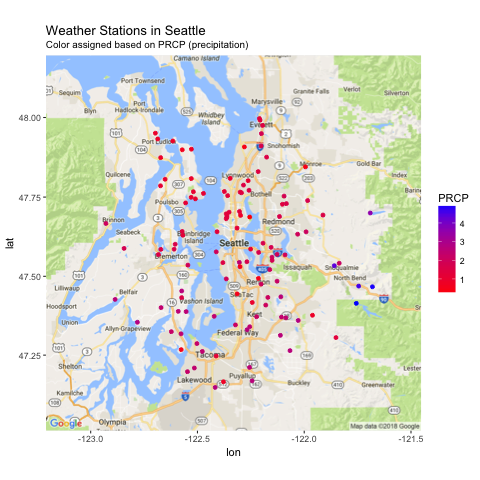
\includegraphics[width=6cm]{station1.png}
\end{minipage}
\begin{minipage}[t]{0.48\textwidth}
\centering
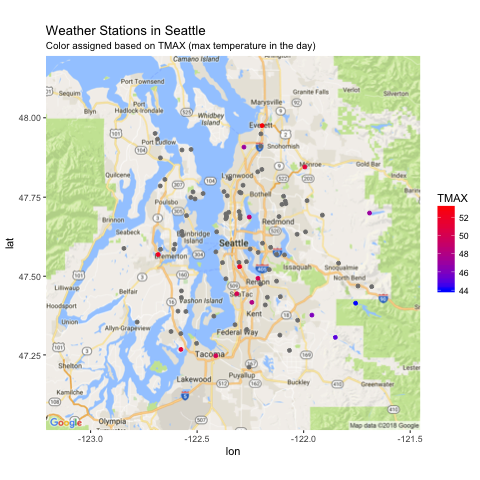
\includegraphics[width=6cm]{station2.png}
\end{minipage}
\caption{Station Positions}
\label{pos}
\end{figure}